%!TEX root = ./main.tex
\section{Groups}
\subsection{Groups}
There are two definitions to define a group.
\begin{definition}[Concrete definition]
	A group is a symmetries of something 1:1 map preserving ``structure''.
\end{definition}
\begin{example}
	Consider the rotation of a rectangle, we have a group of order $4$.
\end{example}
\begin{example}
	Consider the rotation of a icosahedron, we are able to obtain a group of order $60$.
\end{example}
\begin{example}
	Let $V$ be a $n$-dimensional over $\b R$. The general linear group $GL_n(\b R)$, all matrices with $\det \neq 0$ from a group. 
\end{example}
\begin{definition}[Abstract Definition, Cayley]
	A group is a set $G$ with a binary operation $a + b$ or $a \times b$ or $a \circ b$ or $ab$ (notation sucks) such that
	\begin{enumerate}
		\item Identity element $0$, $1$, or $e$, i,e $a1 = 1a = a$.
		\item Each element has inverse $a^{-1}$, i,e $aa^{-1} = a^{-1}a = 1$.
		\item Associative $(ab)c = a(bc)$ for all $a,b,c \in G$
	\end{enumerate}
\end{definition}
\begin{definition}
	A group $G$ acts on $S$ means given operation 
	\[ G \times S \to S \]
	such that $1s = s$ and $a(bs) = ab(s)$.
\end{definition}
\begin{example}
	Let $G$ be the icosahedron group and let $S$ be the icosahedron.
\end{example}
\begin{question}
	How does $G$ acts on $G$?
\end{question}
\begin{definition}
	There are 8 different types of actions
	\begin{enumerate}
		\item $g(s) = s$, left action (trivial)
		\item $g(s) = gs$
		\item $g(s) = sg^{-1}$
		\item $g(s) = gsg^{-1}$, adjoint action
	\end{enumerate}
	Note that all of these are left actions of the group, then similarly there are also 4 right group actions. $S \times G \to S$
	\begin{enumerate}
		\item $sg = s$
		\item $sg = sg$
		\item $sg = g^{-1} s$
		\item $sg = g^{-1}sg$
	\end{enumerate}
\end{definition}
\begin{remark}
	$g(s) = gs, g(s) = sg^{-1}, sg = sg, sg = g^{-1}s$ does not preserve group operation of $S$.
\end{remark}
We let $G$ act on $S(=G)$ by $g(s) = gs$. This means $G$ into subset of all permutations of $S(=G)$. Now we want to add extra ``structure'' to $S$ so $G$ is exactly symmetries of $S$ with this structure.

Extra structure is \textbf{right} action of $G$ on $S$. We now have 3 copies of $G$
\begin{enumerate}
	\item Set $S(=G)$.
	\item $G$ acting on \textbf{right} on $S$ $\leftarrow$ part of structure
	\item $G$ acting on \textbf{left} on $S$ $\leftarrow$ symmetry group
\end{enumerate}
\begin{example}[Cayley Graph of 4 elements]
	$ $
	\begin{center}
		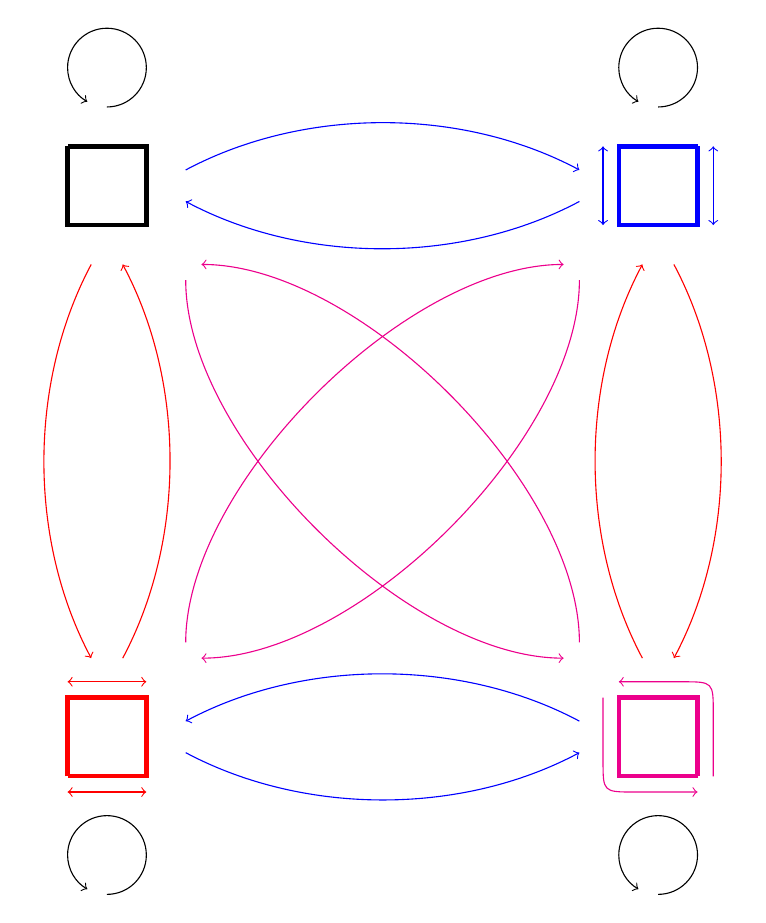
\begin{tikzpicture}
		\draw[color = blue, ultra thick] (4,4)--(4,3)--(3,3)--(3,4)--(4,4);
		\draw[color = red, ultra thick] (-4,-4)--(-4,-3)--(-3,-3)--(-3,-4)--(-4,-4);
		\draw[color = magenta, ultra thick] (4,-4)--(4,-3)--(3,-3)--(3,-4)--(4,-4);
		\draw[ultra thick] (-4,4)--(-4,3)--(-3,3)--(-3,4)--(-4,4);
		\draw[->] (3.5,4.5) arc (270:600:0.5);
		\draw[->] (-3.5,4.5) arc (270:600:0.5);
		\draw[->] (3.5,-5.5) arc (270:600:0.5);
		\draw[->] (-3.5,-5.5) arc (270:600:0.5);
		\draw[<->, color = blue] (4.2,3) -- (4.2,4);
		\draw[<->, color = blue] (2.8,3) -- (2.8,4);
		\draw[<->, color = red] (-4,-2.8) -- (-3,-2.8);
		\draw[<->, color = red] (-4,-4.2) -- (-3,-4.2);
		\draw[->, color = magenta] (2.8,-3) -- (2.8,-3.8) .. controls (2.8,-4.2) .. (3.2,-4.2) -- (4,-4.2);
		\draw[->, color = magenta] (4.2,-4) -- (4.2,-3.2) .. controls (4.2,-2.8) .. (3.8,-2.8) -- (3,-2.8);
		\draw[->, color = magenta] (2.5,2.3) .. controls +(down:20mm) and +(right:20mm) .. (-2.3,-2.5);
		\draw[->, color = magenta] (-2.5,-2.3) .. controls +(up:20mm) and +(left:20mm) .. (2.3,2.5);
		\draw[->, color = magenta] (2.5,-2.3) .. controls +(up:20mm) and +(right:20mm) .. (-2.3,2.5);
		\draw[->, color = magenta] (-2.5,2.3) .. controls +(down:20mm) and +(left:20mm) .. (2.3,-2.5);
		\draw[->, color = blue] (2.5,3.3) .. controls (1,2.5) and (-1,2.5) .. (-2.5,3.3);	
		\draw[<-, color = blue] (2.5,3.7) .. controls (1,4.5) and (-1,4.5) .. (-2.5,3.7);	
		\draw[->, color = blue] (2.5,-3.3) .. controls (1,-2.5) and (-1,-2.5) .. (-2.5,-3.3);	
		\draw[<-, color = blue] (2.5,-3.7) .. controls (1,-4.5) and (-1,-4.5) .. (-2.5,-3.7);
		\draw[->, color = red] (3.7,2.5) .. controls (4.5,1) and (4.5,-1) .. (3.7,-2.5);
		\draw[<-, color = red] (3.3,2.5) .. controls (2.5,1) and (2.5,-1) .. (3.3,-2.5);
		\draw[->, color = red] (-3.7,2.5) .. controls (-4.5,1) and (-4.5,-1) .. (-3.7,-2.5);
		\draw[<-, color = red] (-3.3,2.5) .. controls (-2.5,1) and (-2.5,-1) .. (-3.3,-2.5);
		\end{tikzpicture}
	\end{center}
	We get colored (directed) graph arrow gives \textbf{right} action of $G$, which is not the same as the \textbf{left} action.
\end{example}
\begin{remark}
	Goals of group theory
	\begin{enumerate}
		\item Classify all groups
		\item Given a group $G$, find all ways $G$ acts on something.
	\end{enumerate}
\end{remark}
\begin{example}
	Linear representation = actions of $G$ over vector space.

	Permutation = actions of $G$ over on a set.
\end{example}
\begin{definition}
	A homomorphism $f: G \to H$ map preserving group structure. i.e. $f(gh) = f(g)f(h)$.

	A isomorphism is a homomorphism that is a bijection. 

	The kernel of $f$ is the set of elements such that it maps to the trivial element of $H$ 
\end{definition}
\begin{example}
	Consider the function
	\[ \mathrm{exp} : \langle \b R, + \rangle \to \langle \b R^*, \cdot \rangle\]
	exp is a isomorphism from $\b R$ to $R_{> 0}$
\end{example}
\begin{example}
	Consider the function
	\[ \mathrm{exp} : \langle \b C, + \rangle \to \langle \b C^*, \cdot \rangle\]
	kernel = elements $2\pi i n, n \in \b Z$.
\end{example}
\begin{example}[Number Theory]
	Consider $\b Z/4 \b Z$ integers mod $4$. and $\left( \b Z/ 5 \b Z \right)^*$ nonzero integers mod $5$ under multiplication.
\end{example}
\begin{example}
	Consider the function :
	\[ \mathrm{det} : GL_n(R) = \b R^*\]
	is a homomorphism.

	kernel = $SL_n(\b R)$ = special linear group.
\end{example}
\begin{theorem}[Lagrange's Theorem]
	If $H$ is a subgroup of $G$, order of $H$ divides order of $G$. ($G$ is finite)
\end{theorem}
\begin{lemma}
	2 cosets either are the same or disjoint.
\end{lemma}
\begin{proof}
    If $aH \cap bH = \varnothing$, then the proof is done. \\
    Now we suppose $aH \cap bH \neq \varnothing$, then we know that $ah_1 = bh_2$ for some element in $aH$ and $bH$. We compute $ah_1 = bh_2 \implies h_1 = a^{-1}bh_2 \implies a^{-1}b = h_1h_2^{-1} \implies a^{-1}b \in H$. By proposition 1 we know that $aH = bH$. \\
    We can use a similar argument to show that this works for the right cosets as well. This is left as an exercises to the reader. 
\end{proof}
\begin{lemma}
	Any cosets have the same size.
\end{lemma}
\begin{proof}
    We can simply prove that $\phi: h \mapsto bh$ is bijective, therefore $|H| = |bH|$. \\
    This proof is trivial and is left as an exercise to the reader. (Hint: prove that $\phi$ is injective and say it's surjective by construction)
\end{proof}
\begin{proof}
	Suppose $G$ acts on $S$. Pick $s \in S$, put $H = $set of elements fixing $s$ such that $hs = s$, then $H$ is a subgroup of $G$.

	Given a subgroup $H$ of $G$, we can find set $S$ acted on by $G$, $s \in S$. $H$ = things fixed in $S$.

	Given $g,h (H \subseteq G)$. $S = $ left cosets of $H$. 

	we get action of $G$ on set of cosets by putting $g(aH) = (ga)H$. (well-defined left as an exercise)

	Therefore $|G| = |H| \times $ number of cosets. Therefore the order of $H$ divides the order of $H$.
\end{proof}
\begin{theorem}
	If $g \in G$, then the order of $g$ divides divides order of $G$.
\end{theorem}
\begin{corollary}
	If $G$ is prime order, it is cyclic
\end{corollary}
\begin{proof}
	Pick any element $g \neq 1$. Order divided $p$, so $p$ is primes. so $G = $ powers of $g$
\end{proof}
\begin{example}
	List of all groups
	\begin{enumerate}
		\item Order 1 : Trivial group
		\item Order 2 : 1 group $\b Z/2\b Z$, $0,1$.
		\item Order prime $p$ : Integer $\mod p$.
		\item Order 4 : Cyclic group $\b Z/4 \b Z$ and symmetry of a rectangle. These are not isomorphic as the symmetry group of rectangle does not have a element of order $4$. 

		\item Classify all groups with $g^2 = 1$ for all $g$. Group is abelian. $gh = hg$. This follows because $ghgh = (gh)^2 = 1 = h^2g^2 = hhgg \implies hg = gh$.
		 Since $G$ is abelian, we can write group operation. Notice that $G$ is a vector space over field of order $2$, namely $\b Z/2 \b Z$. so $h$ has a basis, and is isomorphic to $\left( \b Z/2\b Z\right)^n$($n$-dimensional vector space) to some $n$. So only $1$ other group of order $4$.
	\end{enumerate}
\end{example}
\begin{definition}
	Suppose $G,H$ are groups, then the product(sum) of the group is defined as follows
	\[ G \times H = \text{set of pairs} (g,h) \]
	and the operation is defined as 
	\[ (g_1,h_1)(g_2,h_2) = (g_1g_2,h_1h_2)\]
\end{definition}
\begin{example}
	symmetry of rectangle is isomorphic to $\b Z/2 \b Z \times \b Z/2 \b Z$.
\end{example}
\begin{example}
	$\b C^* = S \times \b R_{>0}$, where $S$ is the circle group. Notice that this is the polar decomposition of complex numbers.
\end{example}
\begin{definition}
	The product(sum) of groups are elements $(g_1, g_2, \ldots)$ such that all but finite number of $g_i$ are trivial.
\end{definition}
\begin{example}
	$\b Q^* = $ infinite sum of groups $\b Z/2 \b Z \times \b Z /3 \b Z \times \b Z /5 \b Z \times \ldots$. This follows by fundamental theorem of arithmetic.
\end{example}